\begin{frame}{The standard model of particle physics}
\begin{figure}
    \centering
    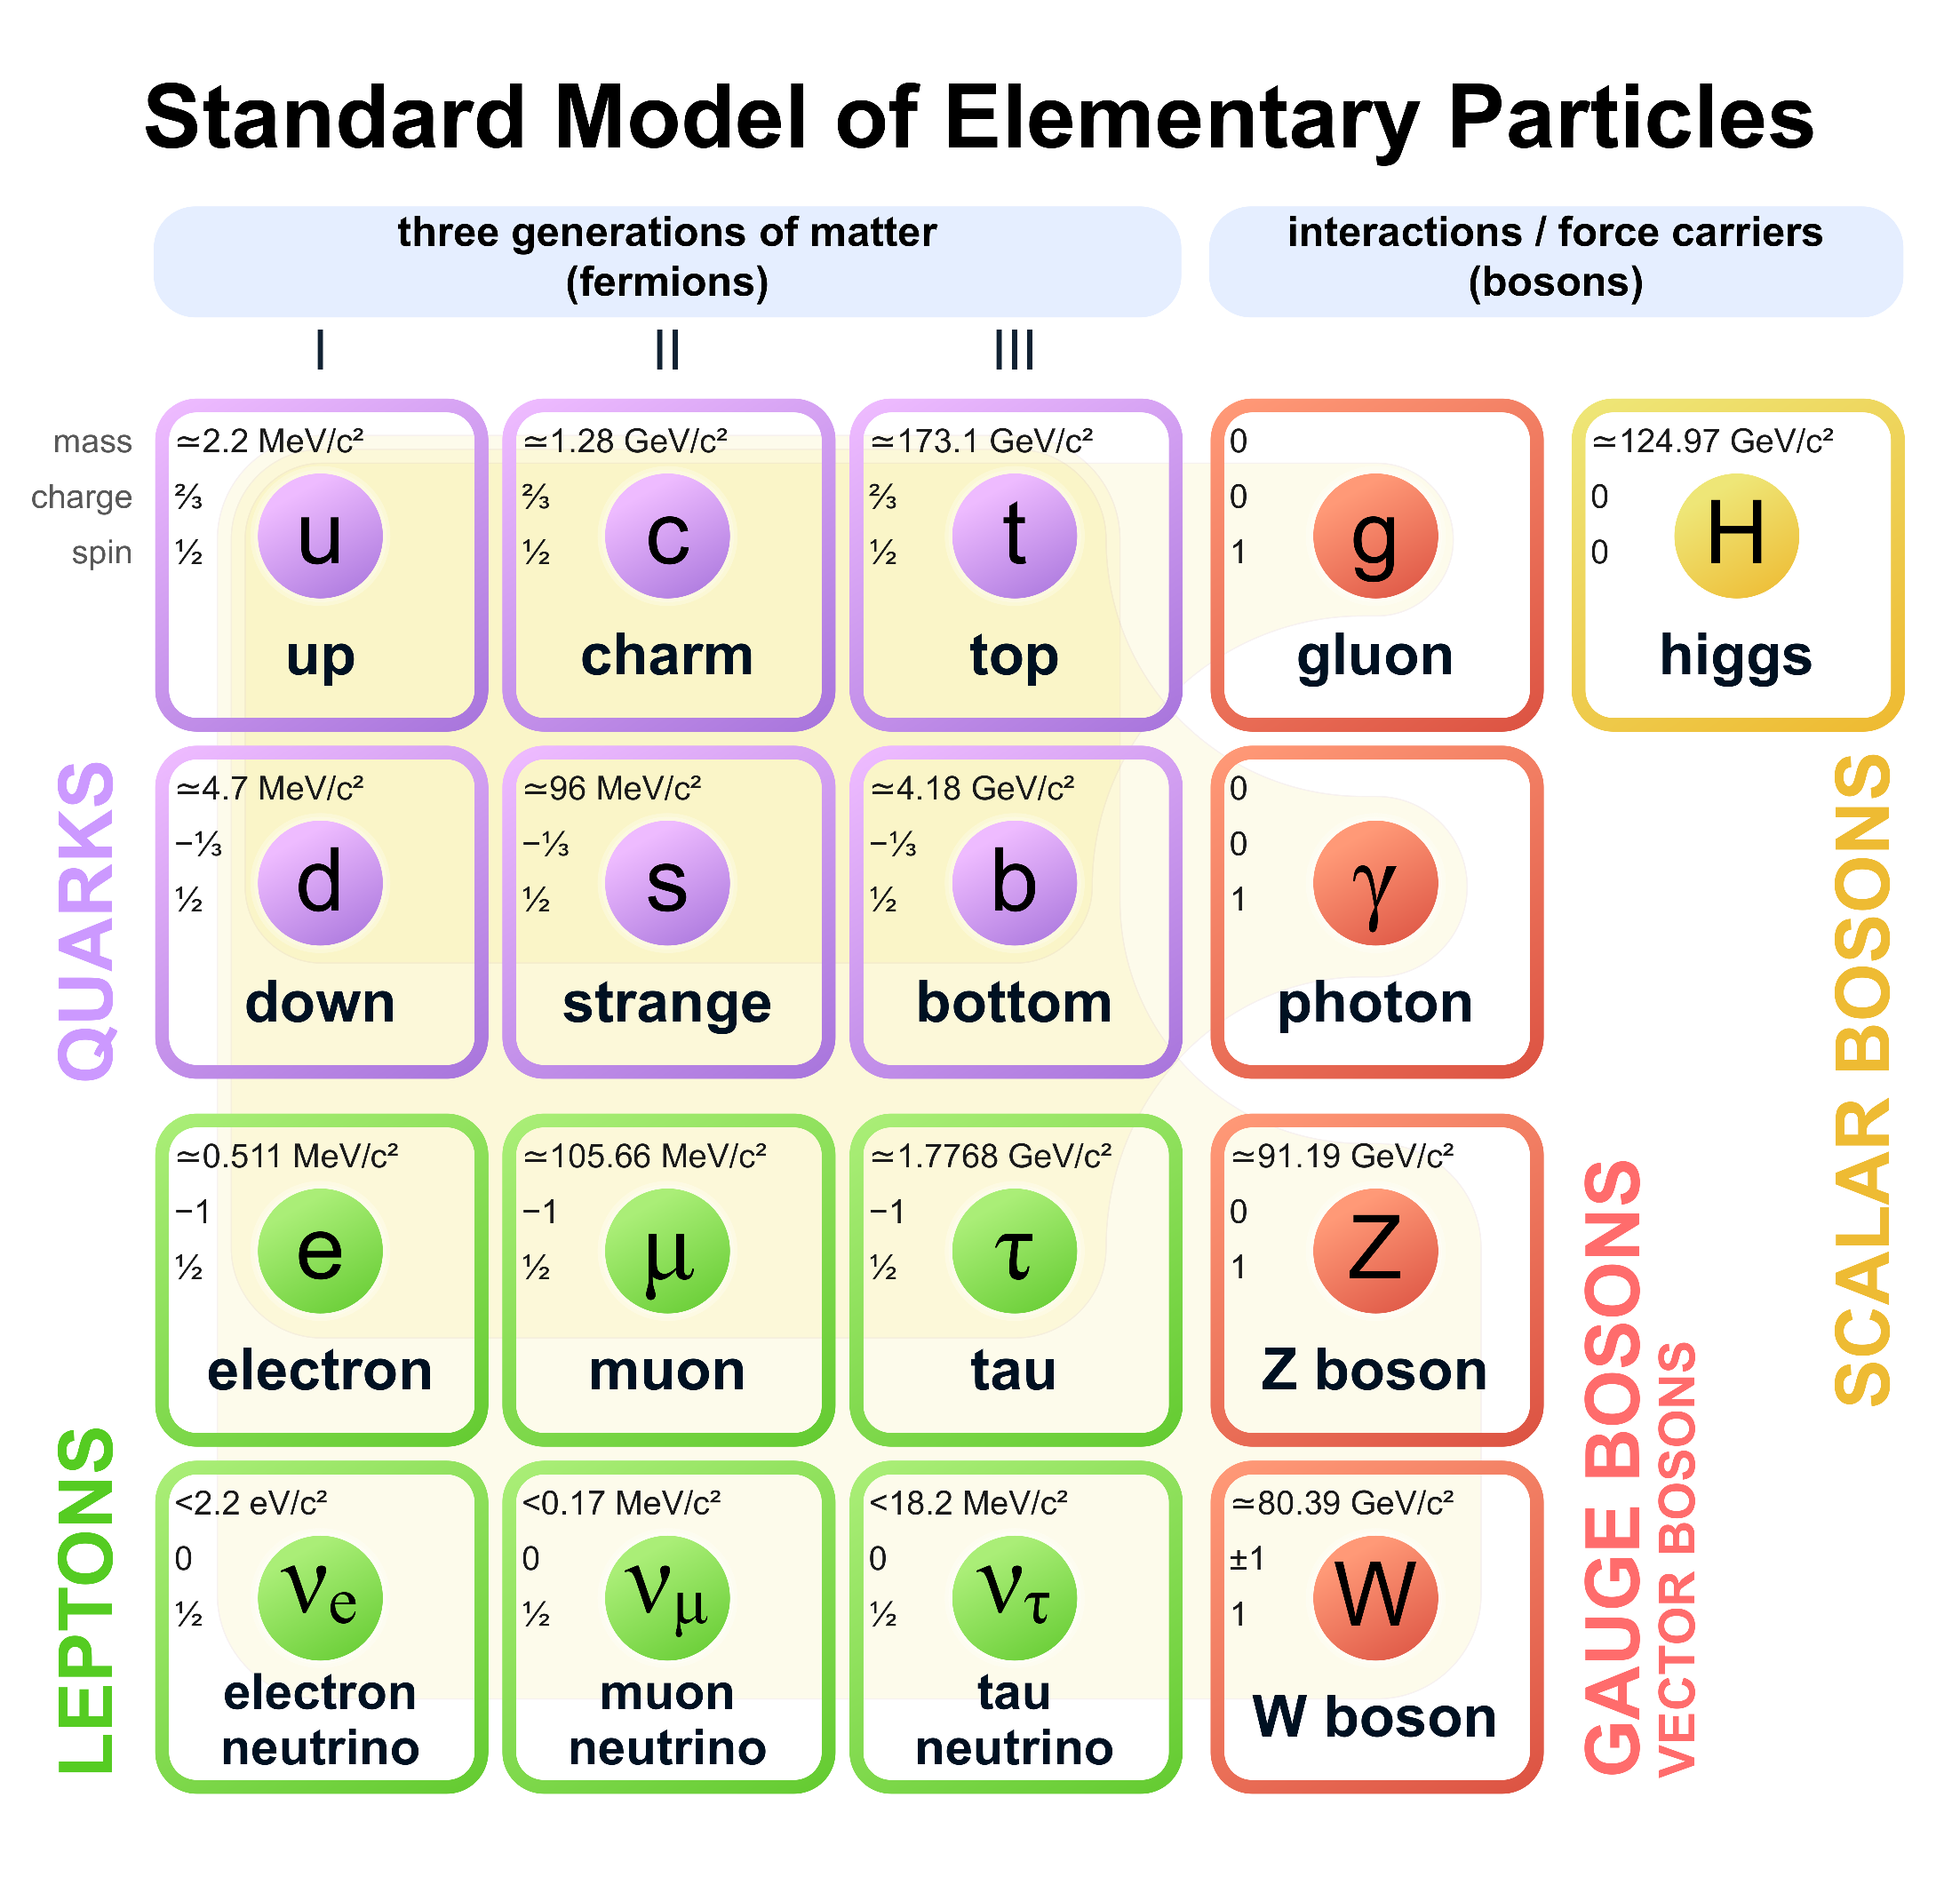
\includegraphics[scale=0.17]{Standard_Model_of_Elementary_Particles.eps}
    \caption{\cite{standard_model}}
    \label{fig:my_label}
\end{figure}
\end{frame}

\begin{frame}{The Large Hadron Collider - LHC}
    \begin{figure}
        \centering
        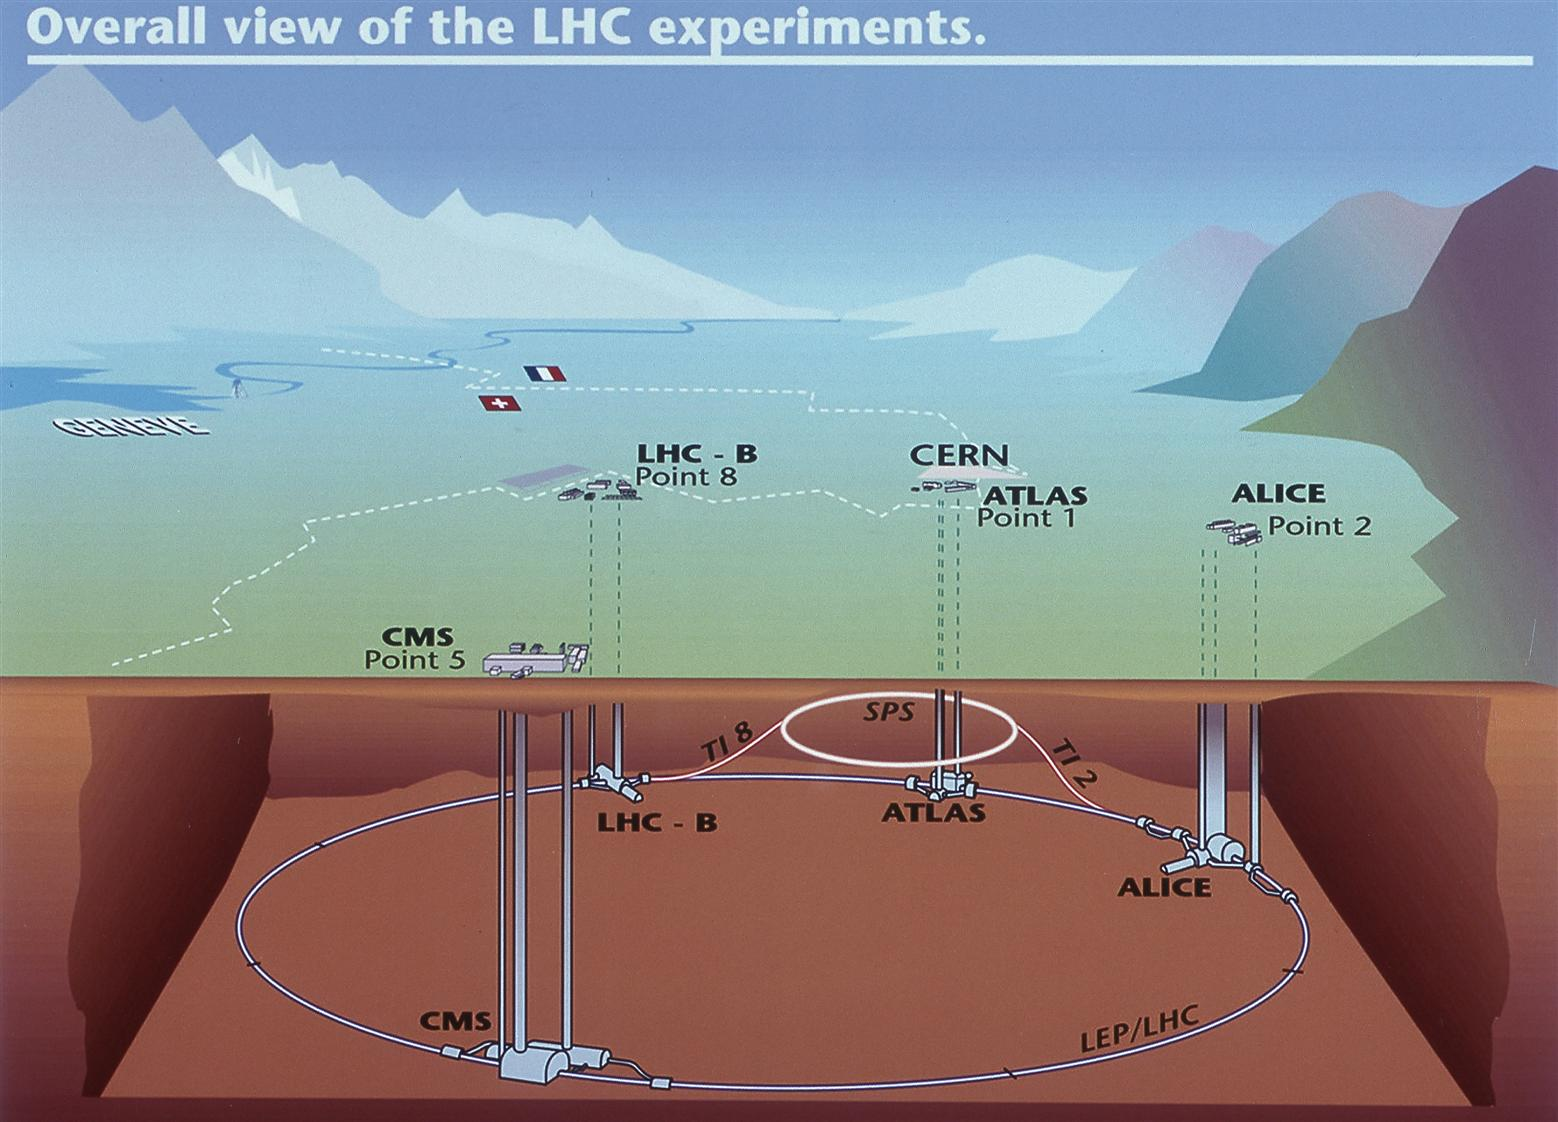
\includegraphics[width=0.6\textwidth]{CERN-all-experiments}
        \caption{\cite{Pequenao:1095924}}
        \label{fig:my_label}
    \end{figure}
     \begin{align*}
        \hfsetfillcolor{logo_blue!10}
        \hfsetbordercolor{logo_blue}
        \tikzmarkin{a1}(0.3,-0.3)(-0.3,0.55)
        E_{CMS} &= \SI{13}{\tera \electronvolt}\\ 
        \mathcal{L} &= \SI{1.5e34}{\per \square \centi \metre  \per \second} 
        \tikzmarkend{a1}
    \end{align*}
\end{frame}

\begin{frame}{The ATLAS experiment}
    \begin{figure}
        \centering
        \includegraphics[width=0.8\textwidth]{lhc_atlas_combination.eps}
        \caption{\cite{Pequenao:1095924}}
        \label{fig:my_label}
    \end{figure}
\end{frame}

\begin{frame}{ATLAS - a genereal purpose detector}
    \begin{figure}
        \centering
        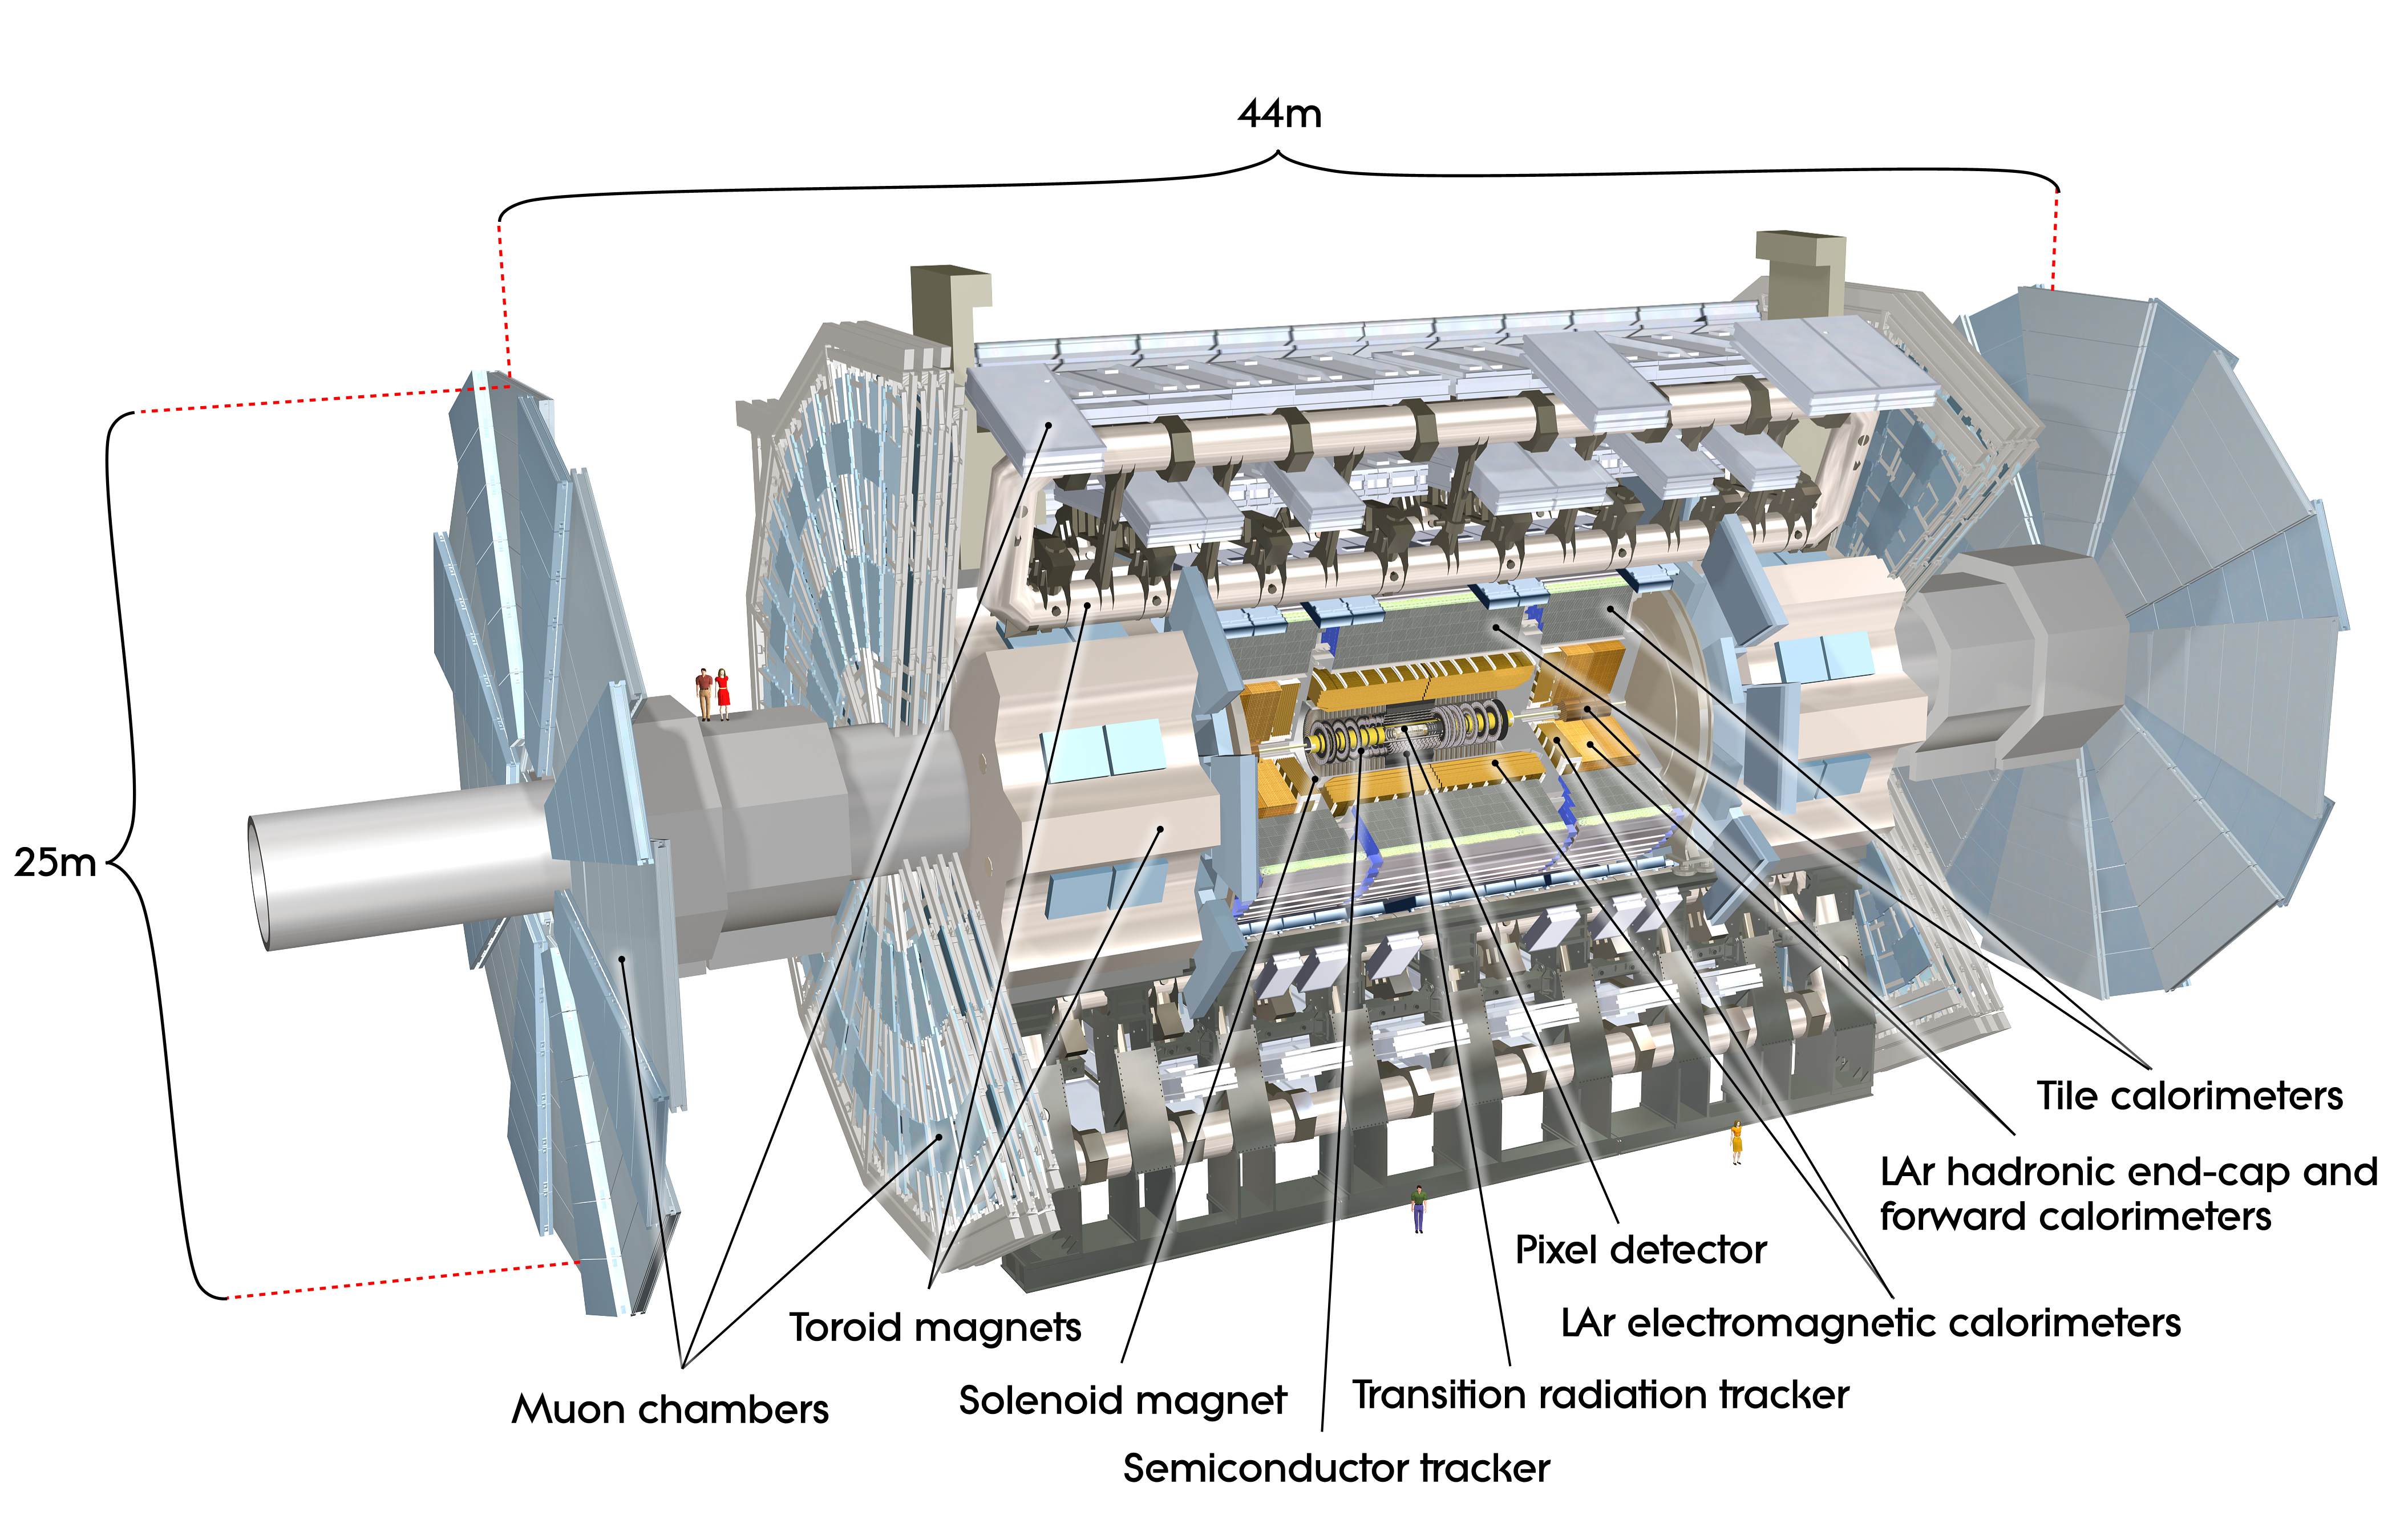
\includegraphics[width=0.8\textwidth]{atlas_detector.jpg}
        \caption{\cite{Pequenao:1095924}}
        \label{fig:my_label}
    \end{figure}
\end{frame}


\begin{frame}{ATLAS - object identification}
    \begin{figure}
        \centering
        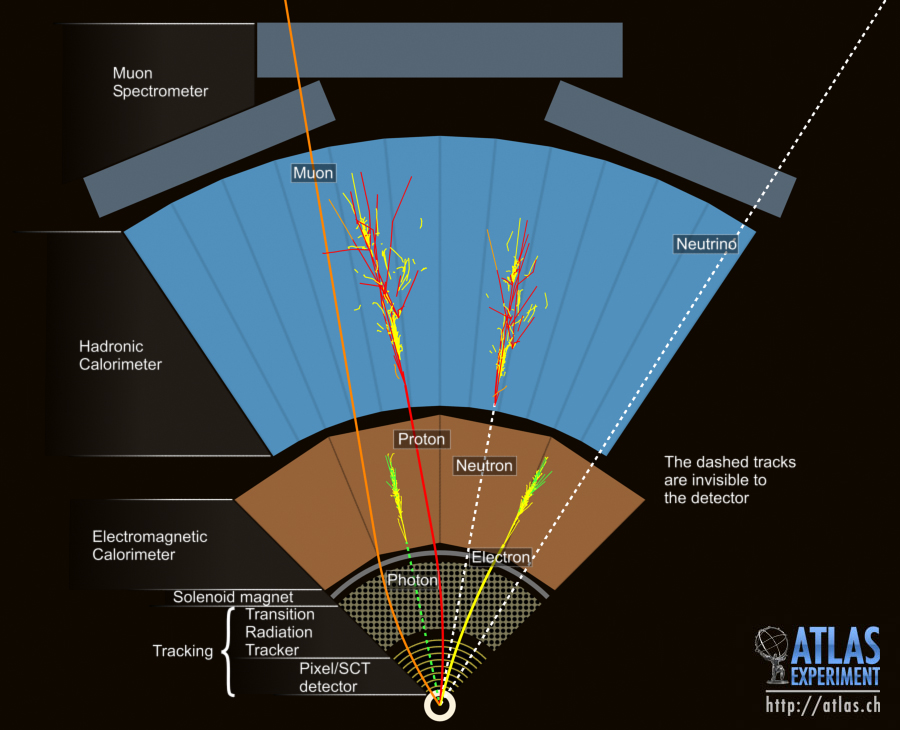
\includegraphics[width=0.8\textwidth]{figures_theory/atlas_quer.jpg}
        \caption{\cite{Pequenao:1095924}}
        \label{fig:my_label}
    \end{figure}
\end{frame}

\begin{frame}{Top physics - The \tW-channel}
    \begin{columns}
        \begin{column}{0.5\textwidth}
        \begin{figure}
            \centering
            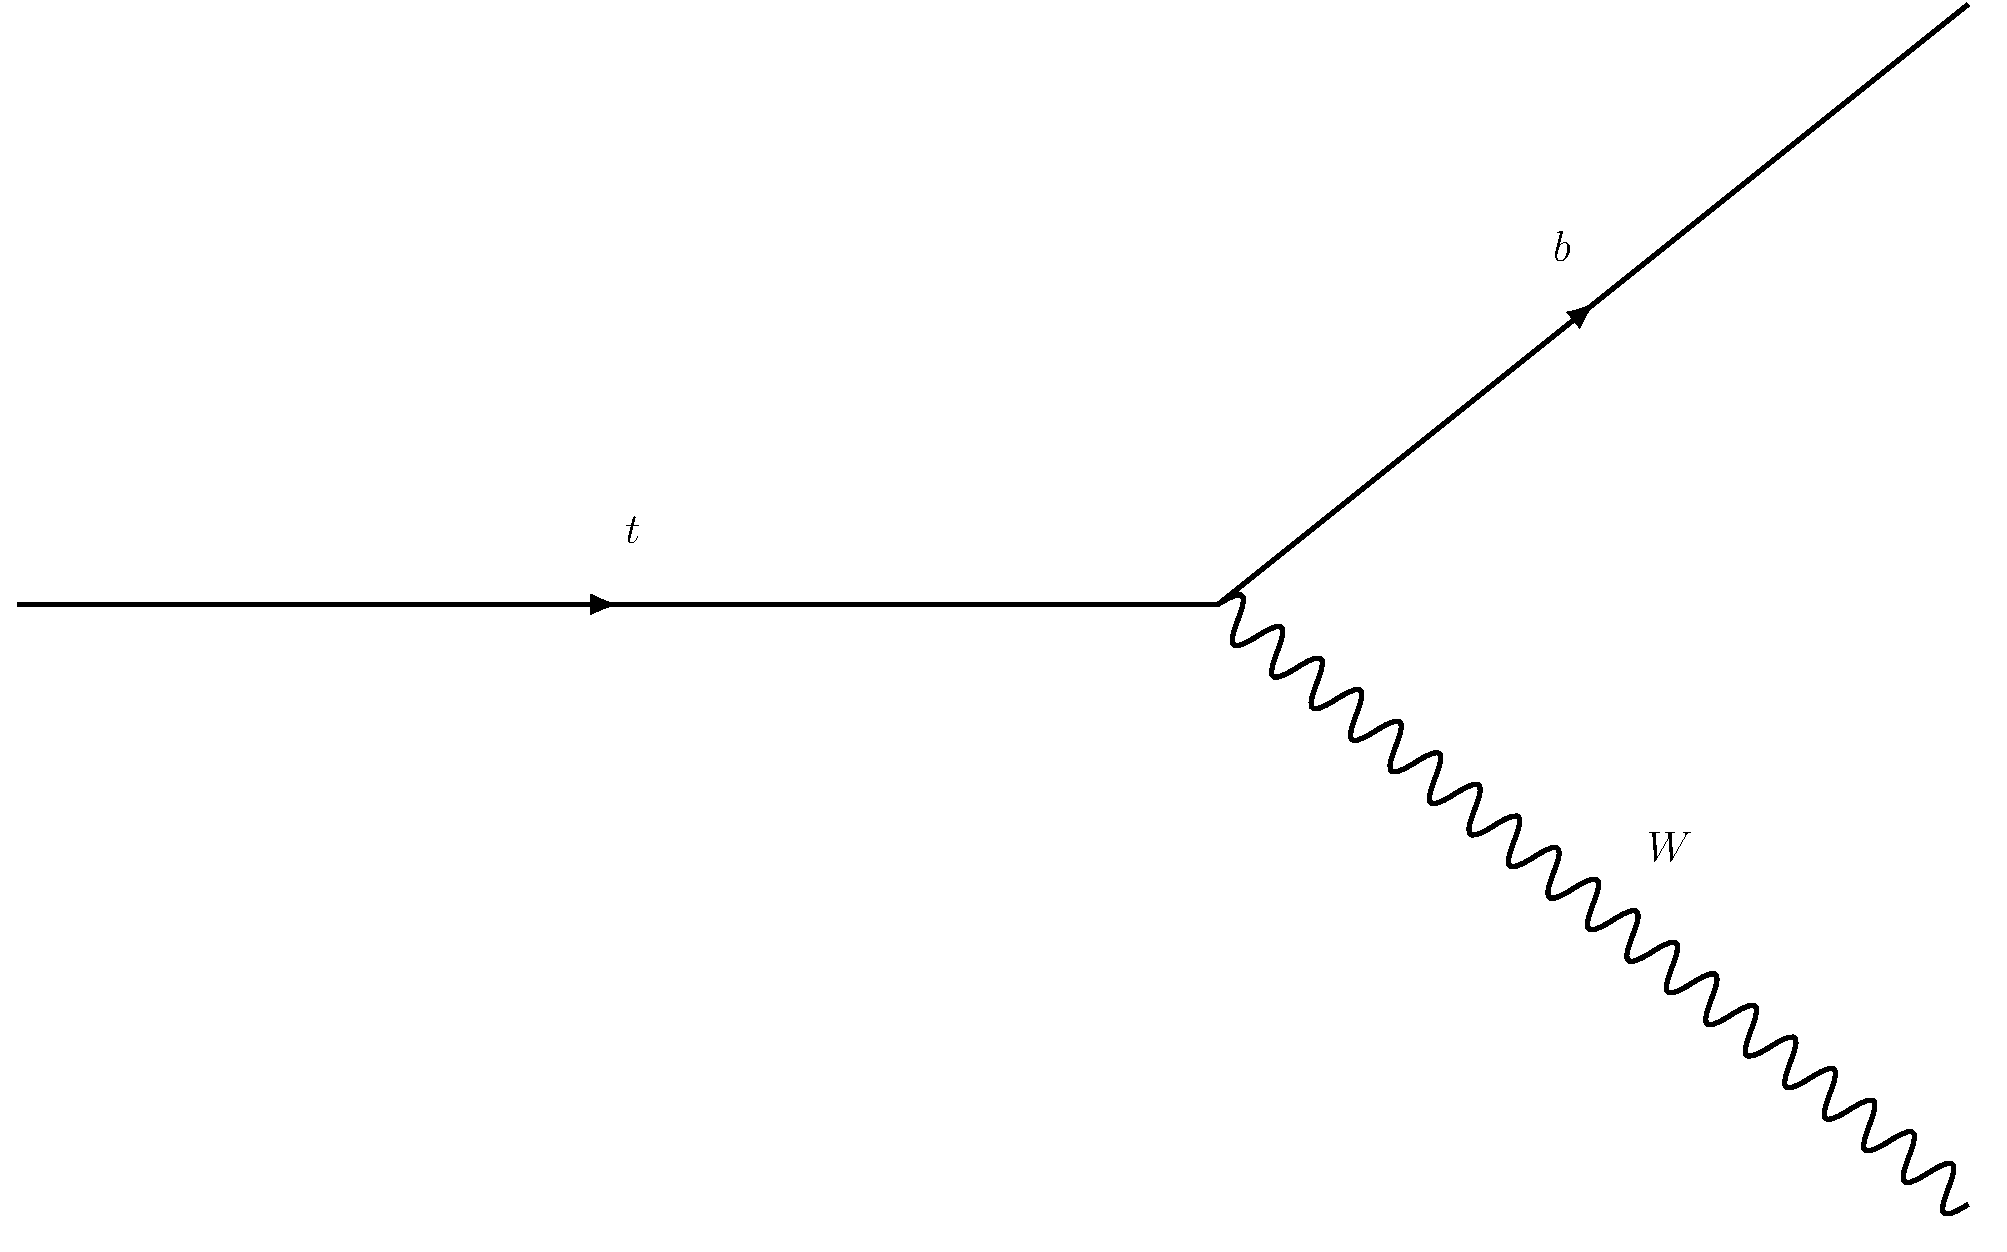
\includegraphics[width=0.8\textwidth]{figures_theory/t_decay.pdf}
        \end{figure}
        \begin{itemize}
            \item $ m \sim \SI{173}{\GeVovercsq}$
            \vspace{0.2cm}
            \item $\tau \sim \SI{5e-25}{\second}$
            \item Decays into a top-quark and a \PW-boson
            \vspace{0.2cm}
            \item Lifetime shorter $<$ typical time of hadronisation 
        \end{itemize}
        \end{column}
        \begin{column}{0.5\textwidth}
        \begin{itemize}
		\item Two production modes
		\item Pair production via strong force
		\item Single top production via electroweak interaction
        \end{itemize}
        \begin{figure}
            \centering
            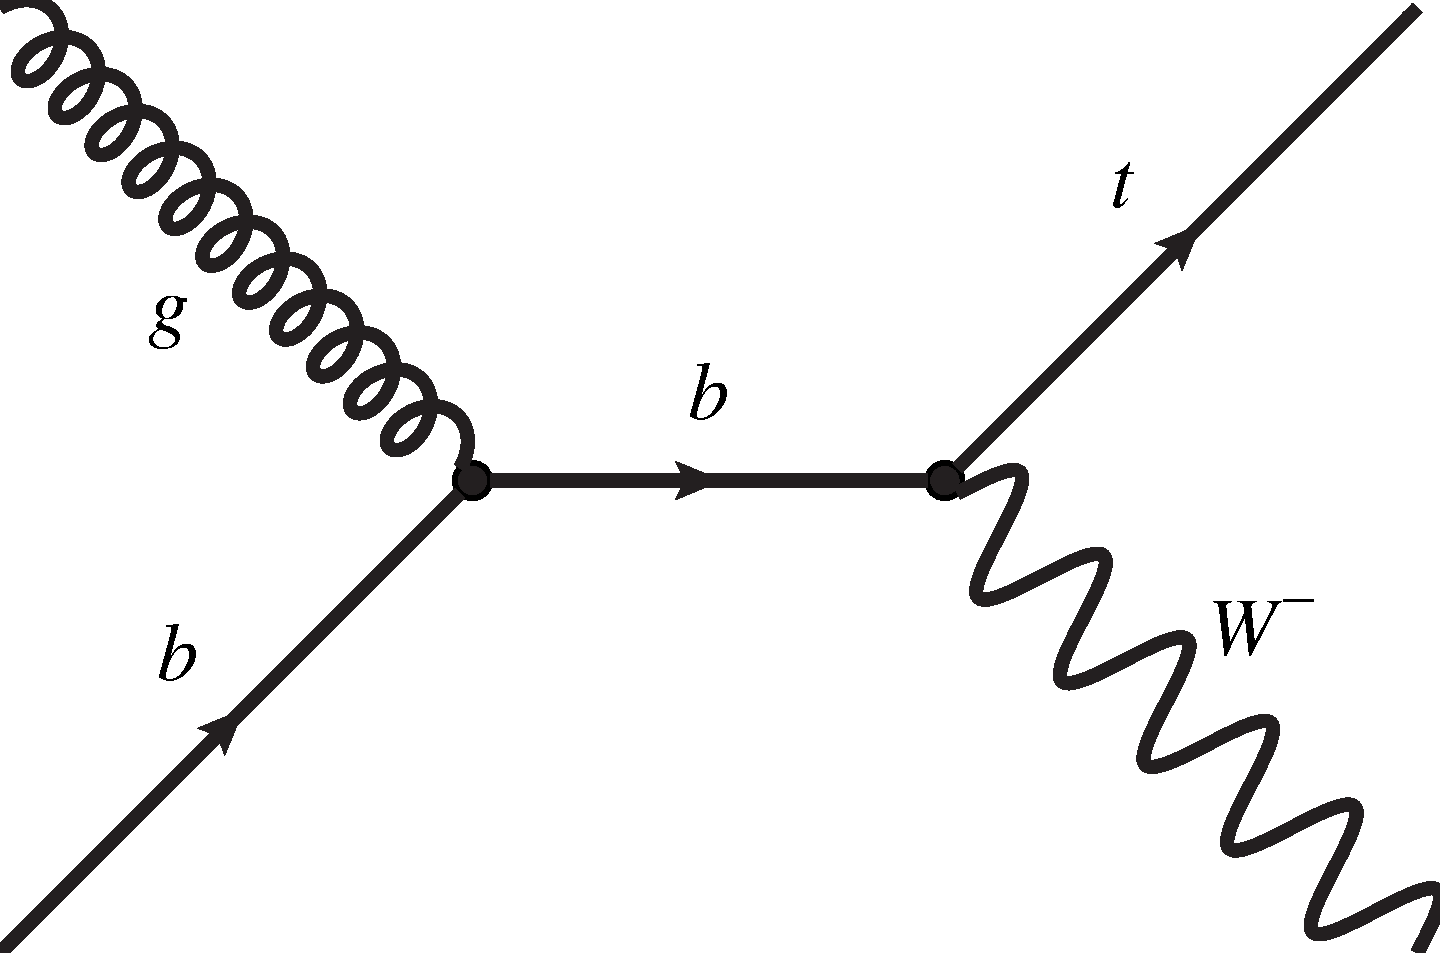
\includegraphics[width=0.8\textwidth]{tW_channel}
        \end{figure}
        \end{column}
    \end{columns}
\end{frame}

\begin{frame}{\tW to \ttbar separation at LO}
    \begin{figure}[htbp]
    \centering
    \begin{subfigure}[b]{0.4\textwidth}
        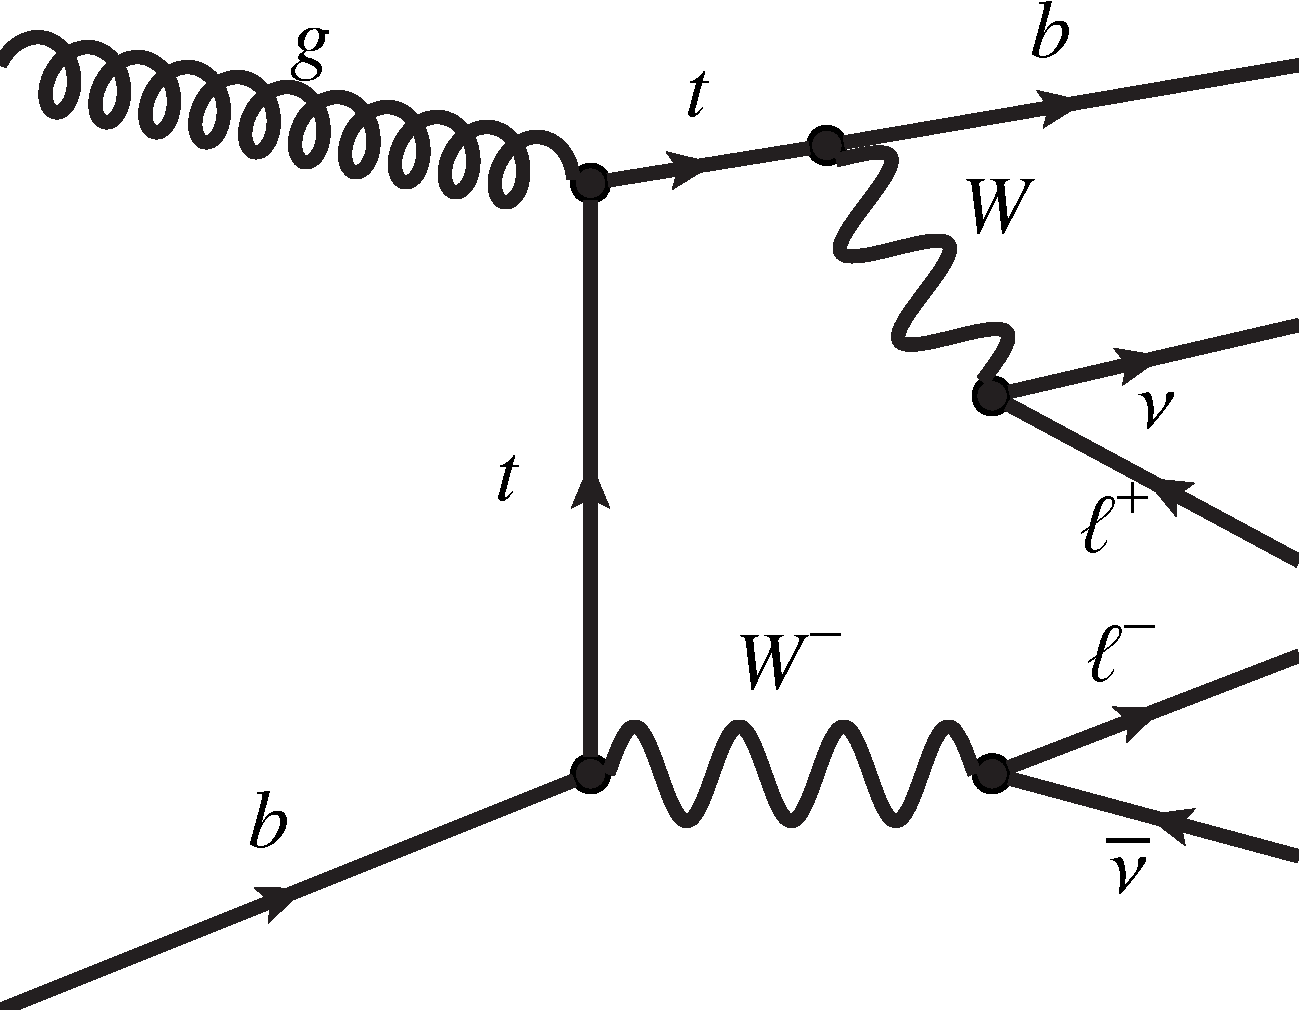
\includegraphics[width=\textwidth]{feynman_diagrams/tW-decay.pdf}
        \label{fig:nlo:tw}
    \end{subfigure}
\quad
    \begin{subfigure}[b]{0.4\textwidth}
        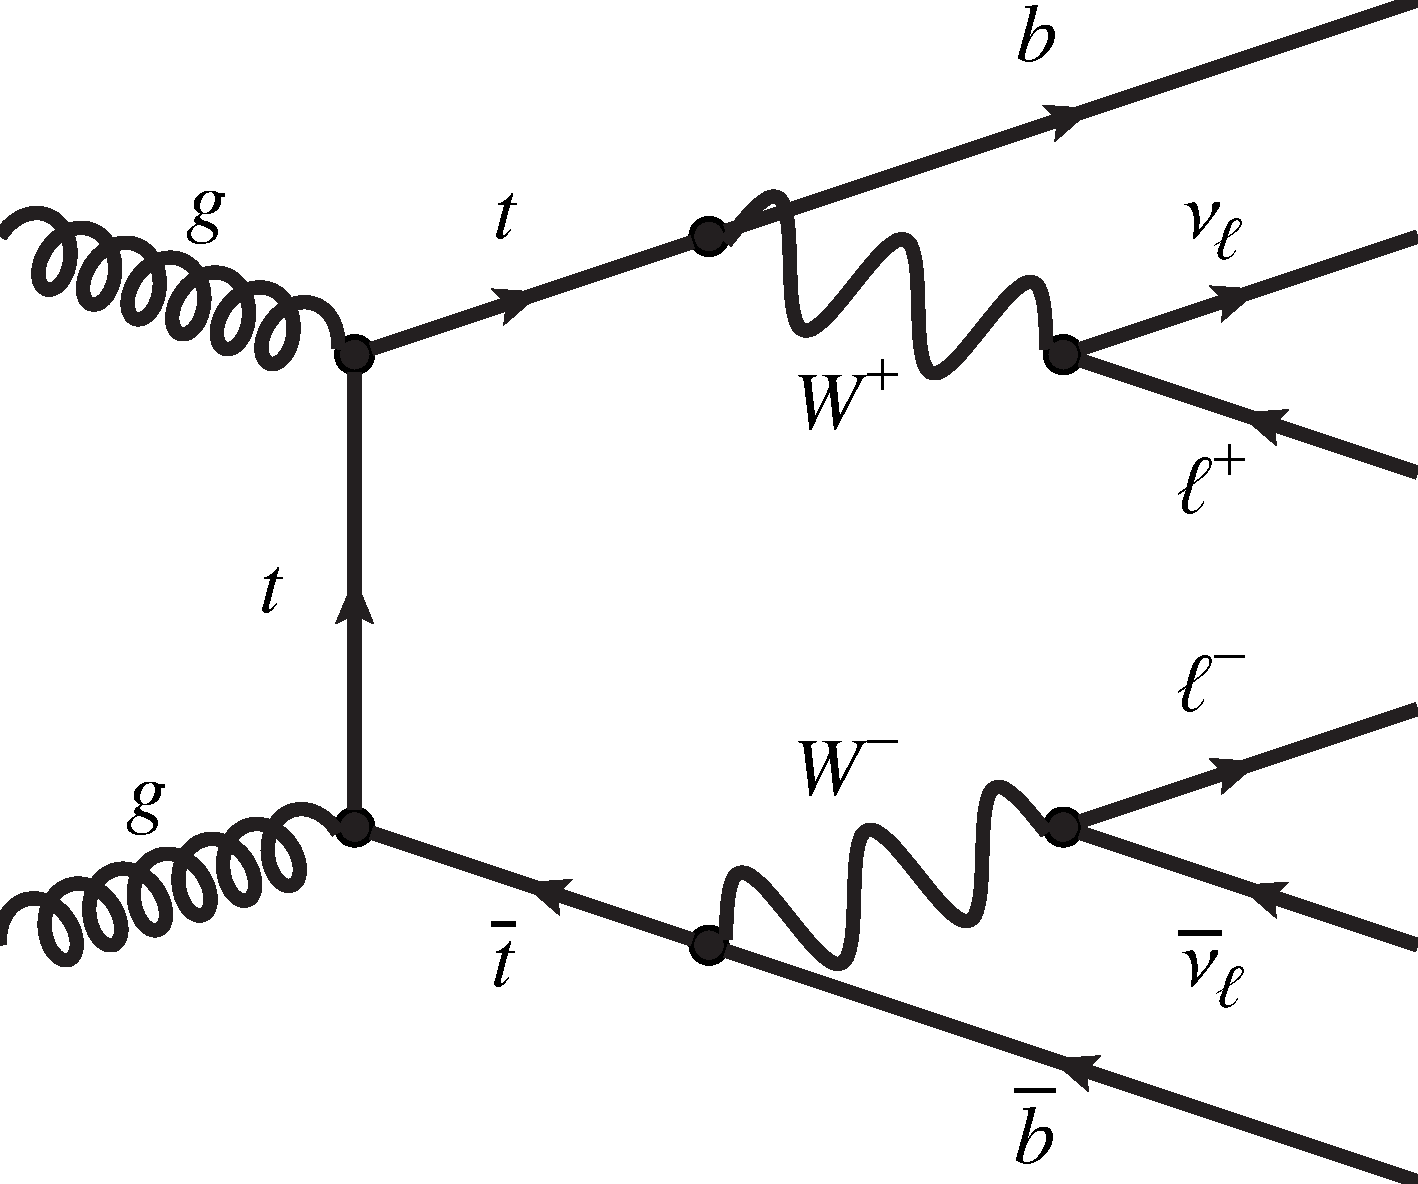
\includegraphics[width=\textwidth]{ttbar-decay}
        \label{fig:nlo:ttbar}
    \end{subfigure}
\end{figure}
%
\begin{columns}
\quad
    \begin{column}{0.45\textwidth}
    \begin{block}{\tW decay}
    $\sigma_{\tW} \sim \SI{71.7}{\pico\barn}$\\
    Final state: 2 \PW, 1 \Pbottom
    \end{block}
    \end{column}
    \quad
    \begin{column}{0.45\textwidth}
    %
    \begin{block}{\ttbar decay}
    $\sigma_{\ttbar} \sim \SI{832}{\pico\barn}$\\
    Final state: 2 \PW, 2 \Pbottom
    \end{block}
    \end{column}
\quad
\end{columns}
\end{frame}

\begin{frame}{\tW to \ttbar separation at NLO}
    \begin{figure}[htbp]
    \centering
    \begin{subfigure}[b]{0.44\textwidth}
        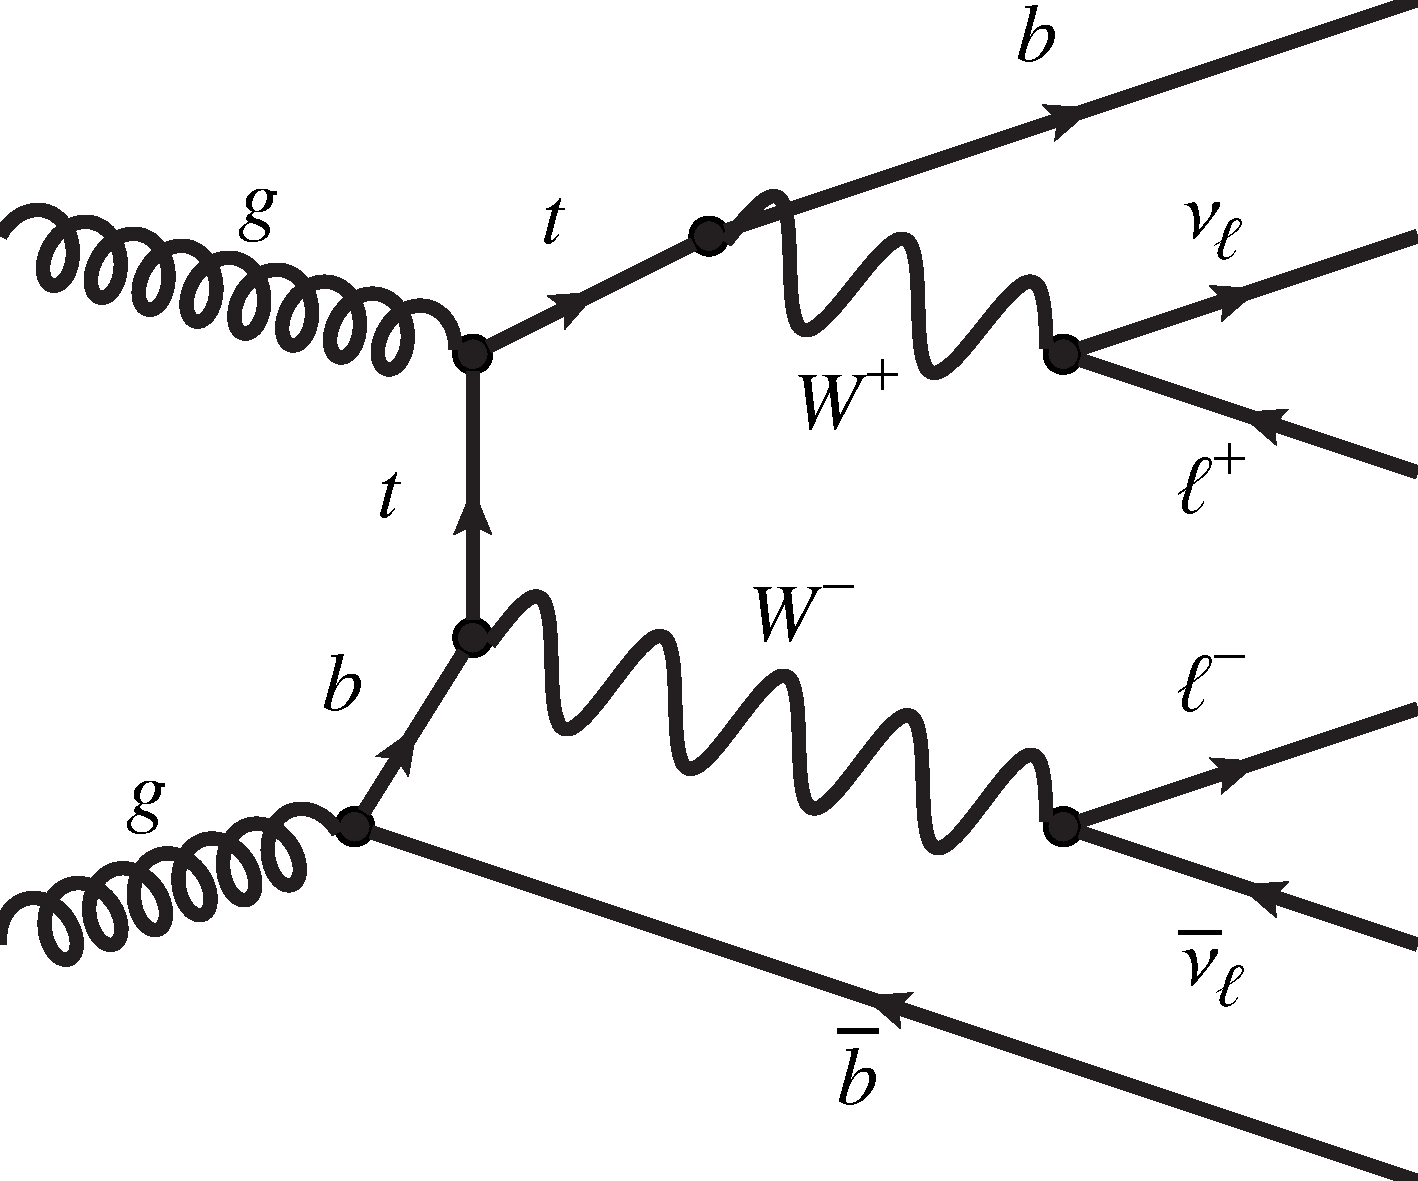
\includegraphics[width=\textwidth]{feynman_diagrams/tw-NLO.pdf}
        %\caption{}
        \label{fig:nlo:ttbar}
    \end{subfigure}
\quad
    \begin{subfigure}[b]{0.44\textwidth}
        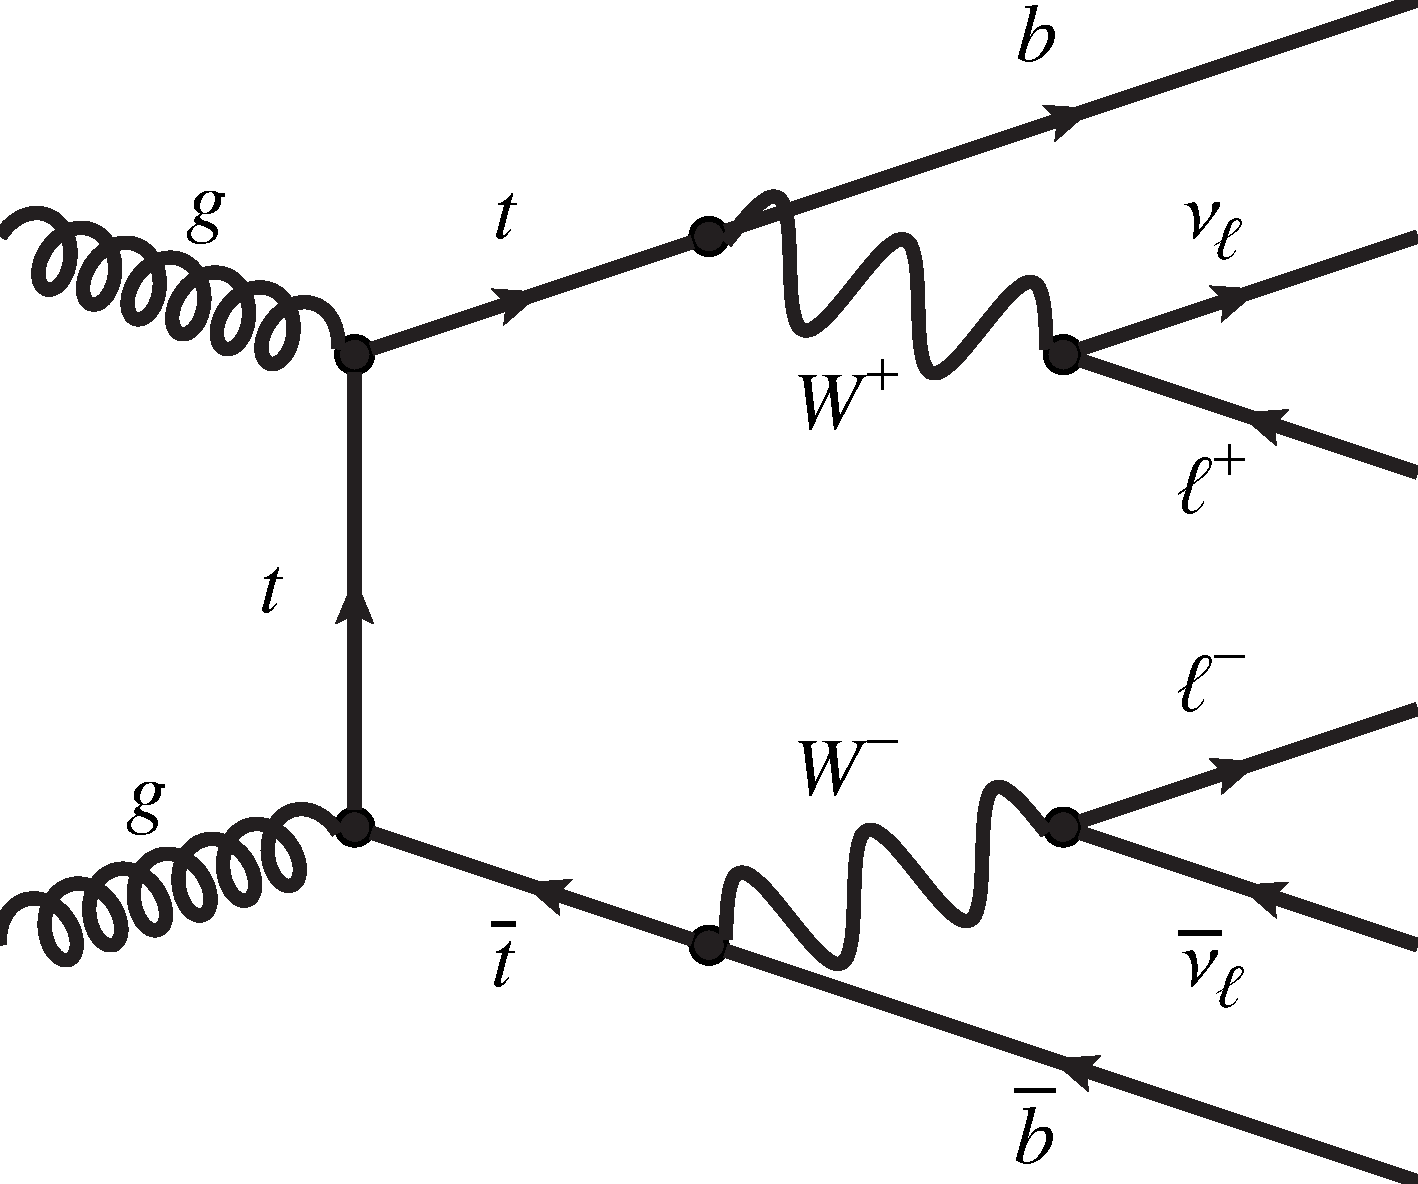
\includegraphics[width=\textwidth]{ttbar-decay}
        %\caption{}
        \label{fig:nlo:tw}
    \end{subfigure}
\end{figure}
%
\begin{columns}
\quad
    \begin{column}{0.45\textwidth}
    \begin{block}{\tW decay at NLO}
    Final state: 2 \PW, 2 \Pbottom
    \end{block}
    \end{column}
    \quad
    \begin{column}{0.45\textwidth}
    %
    \begin{block}{\ttbar decay}
    Final state: 2 \PW, 2 \Pbottom
    \end{block}
    \end{column}
\quad
\end{columns}
\end{frame}
